\documentclass[bachelor, och, otchet, hidelinks]{SCWorks}
% параметр - тип обучения - одно из значений:
%    spec     - специальность
%    bachelor - бакалавриат (по умолчанию)
%    master   - магистратура
% параметр - форма обучения - одно из значений:
%    och   - очное (по умолчанию)
%    zaoch - заочное
% параметр - тип работы - одно из значений:
%    referat    - реферат
%    coursework - курсовая работа (по умолчанию)
%    diploma    - дипломная работа
%    pract      - отчет по практике
%    pract      - отчет о научно-исследовательской работе
%    autoref    - автореферат выпускной работы
%    assignment - задание на выпускную квалификационную работу
%    review     - отзыв руководителя
%    critique   - рецензия на выпускную работу
% параметр - включение шрифта
%    times    - включение шрифта Times New Roman (если установлен)
%               по умолчанию выключен
\usepackage[T2A]{fontenc}
\usepackage[utf8]{inputenc}
\usepackage{graphicx}

\usepackage[sort,compress]{cite}
\usepackage{amsmath}
\usepackage{amssymb}
\usepackage{amsthm}
\usepackage{fancyvrb}
\usepackage{longtable}
\usepackage{array}
\usepackage[english,russian]{babel}
%\usepackage{minted}
% Используется автором репозитория
%\usemintedstyle{xcode}
% Этот пакет включает в себя аналогичный Times New Roman шрифт.
% Необходим для успешной компиляции для UNIX-систем ввиду отсутствия TNR в нем.
% Можно использовать и для Windows.
\usepackage{tempora}


\usepackage[colorlinks=false]{hyperref}

\graphicspath{{figures/}}

\newcommand{\eqdef}{\stackrel {\rm def}{=}}

\newtheorem{lem}{Лемма}

% % При использовании biblatex вместо bibtex
%\usepackage[style=gost-numeric]{biblatex}
%\addbibresource{thesis.bib}

\begin{document}

% Кафедра (в родительном падеже)
\chair{математической кибернетики и компьютерных наук}

% Тема работы
\title{Цифровой компаратор}

% Курс
\course{3}

% Группа
\group{331}

% Факультет (в родительном падеже) (по умолчанию "факультета КНиИТ")
%\department{факультета КНиИТ}

% Специальность/направление код - наименование
%\napravlenie{02.03.02 "--- Фундаментальная информатика и информационные технологии}
%\napravlenie{02.03.01 "--- Математическое обеспечение и администрирование информационных систем}
%\napravlenie{09.03.01 "--- Информатика и вычислительная техника}
%\napravlenie{09.03.04 "--- Программная инженерия}
\napravlenie{10.05.01 "--- Компьютерная безопасность}

% Для студентки. Для работы студента следующая команда не нужна.
%\studenttitle{Студентки}

% Фамилия, имя, отчество в родительном падеже
\author{Бородина Артёма Горовича}

% Заведующий кафедрой
\chtitle{доцент, к.\,ф.-м.\,н.} % степень, звание
\chname{С.\,В.\,Миронов}

%Научный руководитель (для реферата преподаватель проверяющий работу)
\satitle{аспирант}%, к.\,ф.-м.\,н.} %должность, степень, звание
\saname{А.\,А.\,Мартышкин}

% Руководитель практики от организации (только для практики,
% для остальных типов работ не используется)
\patitle{к.\,ф.-м.\,н., доцент}
\paname{Д.\,Ю.\,Петров}

% Семестр (только для практики, для остальных
% типов работ не используется)
\term{2}

% Наименование практики (только для практики, для остальных
% типов работ не используется)
\practtype{учебная}

% Продолжительность практики (количество недель) (только для практики,
% для остальных типов работ не используется)
\duration{2}

% Даты начала и окончания практики (только для практики, для остальных
% типов работ не используется)
\practStart{01.07.2016}
\practFinish{14.07.2016}

% Год выполнения отчета
\date{2022}

\maketitle

% Включение нумерации рисунков, формул и таблиц по разделам
% (по умолчанию - нумерация сквозная)
% (допускается оба вида нумерации)
%\secNumbering


\tableofcontents

% Раздел "Обозначения и сокращения". Может отсутствовать в работе
% \abbreviations
% \begin{description}
%     \item ... "--- ...
%     \item ... "--- ...
% \end{description}

% Раздел "Определения". Может отсутствовать в работе
%\definitions

% Раздел "Определения, обозначения и сокращения". Может отсутствовать в работе.
% Если присутствует, то заменяет собой разделы "Обозначения и сокращения" и "Определения"
%\defabbr


% Раздел "Введение"

\intro

\par Целью данной работы служит ознакомление с основными характеристиками интегрального цифрового 
компаратора и его испытание.

\newpage

\section*{Задание 1.}
\addcontentsline{toc}{section}{Задание 1}

\par Запустить лабораторный комплекс Labworks и среду МS10. Открыть файл \textbf{31.2.ms10}, размещенный в папке
\textbf{Circuit Design Suitе 10.0} среды МS10, или собрать на рабочем поле среды MS10 схему для испытания 
\textit{цифрового компаратора} и установить в диалоговых окнах компонентов их параметры или режимы работы. 
\textbf{Скопировать} схему на страницу отчета.

\begin{figure}[h]
	\center{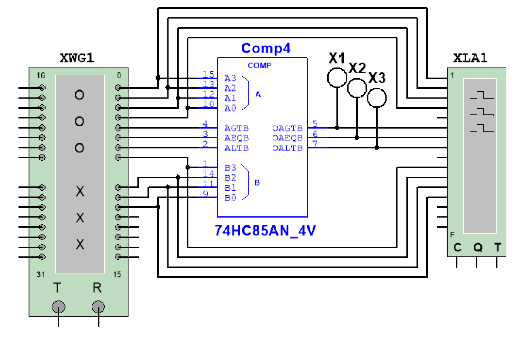
\includegraphics{compar.png}}
	\caption{Схема цифрового компаратора.}
\end{figure}

\newpage

\section*{Задание 2.}
\addcontentsline{toc}{section}{Задание 2}

\textbf{Получить} временные диаграммы входных и выходных сигналов на экране анализатора \textbf{XLA1} при 
пошаговой подаче на входы компаратора сигналов с выходов генератора слова \textbf{XWG1} ($ f_\text{г} $ 
= 500 кГц).

Для этого: 

\par • \textbf{щелкнуть} мышью на изображении генератора \textbf{XWG1} и \textbf{записать} в его первые ячейки 
памяти 10 произвольных 11-разрядных кодовых последовательностей, причем в первые четыре разряда записать 
(справа налево) значения (1 или 0) числа \textbf{А}, то есть А3А2А1А0, в следующие три разряда – 
трехразрядные двоичные числа (\textbf{A} > \textbf{B}, \textbf{A} = \textbf{B} и \textbf{А} < \textbf{B} с 
одним высоким уровнем, равным 1, остальные 0) с выходов предыдущей микросхемы сравнения и, наконец, 
в последние четыре разряда – значения В3В2В1В0 числа \textbf{В}; 

\begin{figure}[h]
	\center{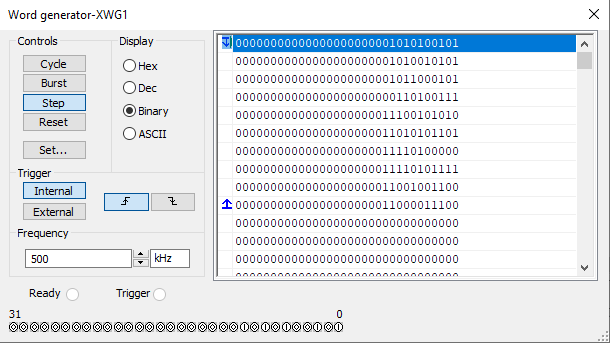
\includegraphics{word_gen.png}}
	\caption{Интерфейс генератора \textbf{XWG1}.}
\end{figure}

\par • \textbf{щелкнуть} мышью на изображении логического анализатора \textbf{XLA1} и \textbf{установить}
в его окне частоту $ f_\text{а} = $ 10 МГц таймера, уровень высокого напряжения $ U_m = $ 4 В и число импульсов 
таймера, приходящихся на одно деление, \textbf{Clocks/div} = 20;

\par • \textbf{запустить} программу моделирования компаратора;

\par • последовательно щелкая мышью на кнопке \textbf{Step} генератора \textbf{XWG1}, \textbf{получить} 
временные диаграммы входных и выходных сигналов на экране анализатора \textbf{XLA1}.

\newpage

\section*{Задание 3.}
\addcontentsline{toc}{section}{Задание 3}

\textbf{Скопировать} на страницу отчета диалоговое окно генератора \textbf{XWG1} и окно анализатора 
\textbf{XLA1} с временными диаграммами входных и выходных сигналов.

\begin{figure}[h]
	\center{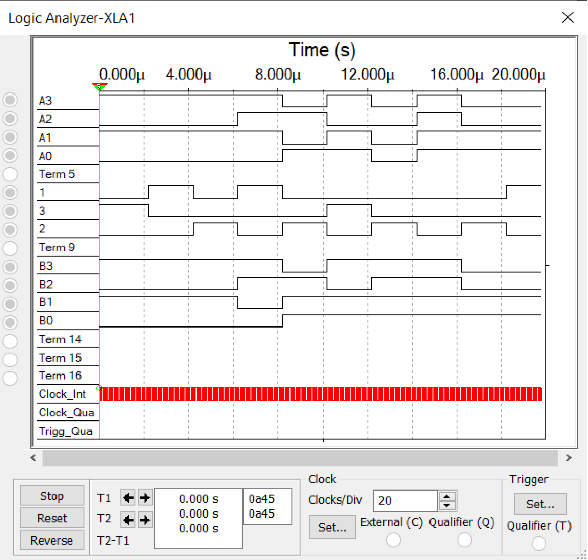
\includegraphics{logic_analyzer.png}}
	\caption{Интерфейс логического анализатора \textbf{XLA1}.}
\end{figure}

\newpage

\section*{Тестовые задания}
\addcontentsline{toc}{section}{Тестовые задания}

\par 1. Укажите:

\par а) можно ли установить \textbf{факт равенства} двухразрядных бинарных чисел \textbf{А} и \textbf{В} с 
помощью приведенного устройства сравнения: \textbf{да}; 

\par б) какой \textbf{уровень} сигнала установится на его выходе при равенстве чисел \textbf{А} и \textbf{В}: 
\textbf{1};

\begin{figure}[h]
	\center{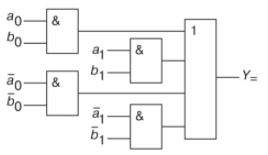
\includegraphics{compar_device.png}}
	\caption{Устройство сравнения двухразрядных бинарных чисел.}
\end{figure}

\par 2. Укажите, какую \textbf{функцию} выполняет цифровой компаратор: сравнение двух бинарных чисел \textbf{А} 
и \textbf{В} одинаковой разрядности с целью определения равенства \textbf{А = В} или неравенства \textbf{А < B} 
и \textbf{A > B};

\par 3. Укажите \textbf{логическую функцию}, выражающую равенство $i-$х разрядов двоичных чисел: 
$ y = a_ib_i + \overline{a}_i \overline{b}_i $;

\par 4. Укажите, к какому \textbf{типу} цифровых устройств относят компараторы: \textbf{к комбинационным};

\par 5. Укажите \textbf{число активных} логических сигналов, формирующихся на выходе компаратора при сравнении 
многоразрядных двоичных чисел: \textbf{1};

\par 6. Укажите, чем определяется \textbf{число входов} цифрового компаратора: \textbf{число входов определяется
разрядностью сравниваемых бинарных чисел}.

\par 7. Укажите, можно ли построить устройство сравнения требуемой разрядности, используя цифровые компараторы 
с ограниченной разрядностью (например, четырехразрядные): \textbf{да}.

\newpage

% Раздел "Заключение"
\conclusion

\par В ходе данной лабораторной работы мы познакомились с основными характеристиками интегрального цифрового
компаратора и испытали его на практике.

\newpage

%Библиографический список, составленный вручную, без использования BibTeX
%
%\begin{thebibliography}{99}
%  \bibitem{Ione} Источник 1.
%  \bibitem{Itwo} Источник 2
%\end{thebibliography}

%Библиографический список, составленный с помощью BibTeX
%
%\bibliographystyle{gost780uv}
%\bibliography{thesis}

% % При использовании biblatex вместо bibtex
%\printbibliography

% Окончание основного документа и начало приложений
% Каждая последующая секция документа будет являться приложением
%\appendix

\end{document}